\documentclass[laboratorio]{guia}

\def \practnum {2} 
\def \practica {Conducci\'on el\'ectrica en l\'\i quidos}

\def \materia {Laboratorio de F\'\i sica II para Qu\'\i micos}
\def \periodo {2do. Cuatrimestre de 2015}
\def \catedra {Pablo Cobelli}
\def \website {http://materias.df.uba.ar/f2qa2015c2}
 
\usepackage{graphics}
\usepackage{amsmath}
\usepackage{amsfonts}
\usepackage{graphicx}
\usepackage{float}
\usepackage{wrapfig}
\usepackage{subfigure}
\usepackage{bm}
\usepackage{grffile}
\usepackage{color}
\usepackage{framed}
\usepackage[utf8]{inputenc}
\usepackage[T1]{fontenc}
\usepackage{lmodern}
\usepackage{circuitikz}
\usepackage[spanish]{babel}
\usepackage{babelbib}
\selectbiblanguage{spanish}

 

%----------------------------------------------------------
% Agrega al path de figuras el subdirectorio con el mismo
%     nombre que el archivo principal del proyecto
\graphicspath{{./\jobname/}}

%----------------------------------------------------------
% Definicion del entorno 'sabermas'
\makeatletter
\definecolor{shadecolor}{rgb}{0.89,0.91,0.94}
\newenvironment{sabermas}[1]{%
\vfill
\begin{shaded}
  \begin{center}
  {\textsection{Para saber m\'as}}
  \end{center}
  #1
\sf } 
{%
\end{shaded}%
}
\makeatother

%----------------------------------------------------------
% Definicion del entorno 'problema'
\newcounter{ContadorProblema}
\setcounter{ContadorProblema}{0}
\newcounter{TieneFiguraAsociada}
\setcounter{TieneFiguraAsociada}{0}
\newcounter{UbicacionFigura}
\setcounter{UbicacionFigura}{0}

\newenvironment{problema}[2][]
{%
    \ifx\relax#1\relax%
        \setcounter{TieneFiguraAsociada}{0}
        \else
        \setcounter{TieneFiguraAsociada}{1}
    \fi
    \def \archivofigura {#1}
    % 
    \refstepcounter{ContadorProblema}
    \noindent%
    \ifnum\value{TieneFiguraAsociada} < 1%
        {\sffamily \bfseries Problema \arabic{ContadorProblema}.}
        %{\sc {#1}}%
        \par\nobreak\par\nobreak%
        \medskip 
    \else
        % Va con figura; resta determinar de que lado.
        \ifnum\value{UbicacionFigura} < 1
            % Poner la figura del lado derecho
            \begin{minipage}{12.25cm}
            {\sffamily \bfseries Problema \arabic{ContadorProblema}.}
            %{\sc {#1}}%
            \par\nobreak\par\nobreak%
            \medskip 
        \else
            % Poner la figura del lado izquierdo
            \begin{minipage}{4.5cm}
                \centering
                \includegraphics[width=4.5cm]{\archivofigura}
                {\footnotesize {\sffamily Esquema asociado al 
                problema \arabic{ContadorProblema}}.}
            \end{minipage}\hfill%
            \begin{minipage}{12.25cm}
                {\sffamily \bfseries Problema \arabic{ContadorProblema}.}
                %{\sc {#1}}%
                \par\nobreak\par\nobreak%
                \medskip 
        \fi
    \fi
}
{%
    \ifnum\value{TieneFiguraAsociada} < 1%
        % \par \bigskip \vskip 0.3cm
    \else
        % Va con figura; resta determinar de que lado.
        \ifnum\value{UbicacionFigura} < 1
            % Poner la figura del lado derecho
            \end{minipage}\hfill%
            \begin{minipage}{4.5cm}
                \centering
                \includegraphics[width=4.5cm]{\archivofigura}
                {\footnotesize {\sffamily Esquema asociado al 
                problema \arabic{ContadorProblema}}.}
            \end{minipage}
        \else
            % Poner la figura del lado izquierdo
            \end{minipage}%
        \fi
    \fi
    \setcounter{TieneFiguraAsociada}{0}
    \par \bigskip \vskip 0.3cm
    % Permutamos el valor de la ubicacion
    \ifnum\value{UbicacionFigura} < 1
        \setcounter{UbicacionFigura}{1}
    \else
        \setcounter{UbicacionFigura}{0}
    \fi
}

%----------------------------------------------------------
% Definicion/Redefinicion de estilos
\renewcommand{\vec}[1]{\ensuremath{\mathbf{#1}}}



\hyphenation{ coe-fi-cien-tes coe-fi-cien-te au-to-va-lor
              au-to-va-lo-res co-rres-pon-der pro-ble-ma 
              cual-quie-ra po-la-ri-za-cio-nes }

\graphicspath{{./Guia_02b_Conduccion_Liquidos/}}

\begin{document} 
\objetivo{%
    El objetivo de esta gu\'\i a experimental es estudiar si los l\'\i quidos
    conducen o no la electricidad. Para aquellos que efectivamente conducen la
    electricidad, se propone estudiar la relaci\'on entre diferencia de
    tensi\'on y corriente, a fin de establecer si satisfacen o no la Ley de
    Ohm. 
    \tematicas{Conducci\'on, corriente, ley de Ohm, materiales \'ohmicos y
        no-\'ohmicos.}} 
\maketitle

\section{Introducci\'on}

Para que un medio material pueda conducir la corriente el\'ectrica \'este debe
contener cargas m\'oviles capaces de conducir la electricidad. En los metales,
las cargas m\'oviles son los mismos electrones de las capas m\'as externas de
los \'atomos que lo forman (electrones de conducci\'on). Al formarse el metal,
el campo de cada \'atomo afecta a sus vecinos m\'as pr\'oximos, lo que hace que
los electrones m\'as externos dejen de estar ligados a un solo \'atomo y tengan
libertad de moverse a trav\'es de todo el s\'olido. En algunos l\'\i quidos,
por ejemplo el agua, si se disuelven sales, \'acidos o bases, \'estas se
disocian en iones positivos y negativos que pueden moverse a trav\'es del l\'\i
quido, por lo que la conducci\'on el\'ectrica se hace apreciable.

\section{Desarrollo de la experiencia; Parte 1}

El dispositivo experimental propuesto para el desarrollo de esta pr\'actica se
ilustra esquem\'aticamente en la Figura~\ref{fig:1}. La tensi\'on que
suministra la fuente de tensi\'on alterna (?`qu\'e es una fuente de tensi\'on
alterna?) es medida por un volt\'\i metro conectado en paralelo. Su valor puede
variarse hasta 20 V. 

\begin{figure}
    \centering
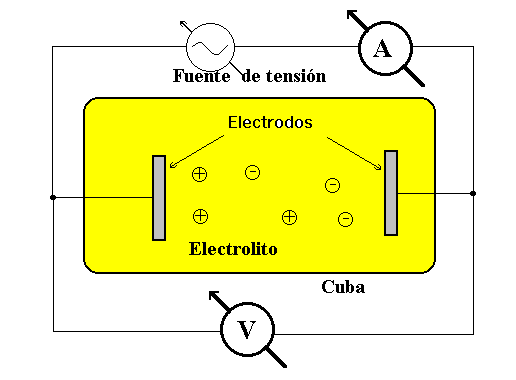
\includegraphics[width=8.5cm]{LG02b--001.png}
\caption{Esquema del dispositivo experimental propuesto (bandeja en vista
superior). La bandeja de material aislante contiene el electrolito bajo
estudio. La fuente suministra una diferencia de tensi\'on alterna de amplitud
controlable. Con V se indica al volt\'\i metro, y con A al amper\'\i metro.}
\label{fig:1}
\end{figure}

Para verificar lo mencionado en la introducci\'on, pruebe aplicando una
tensi\'on alterna a una soluci\'on salina de agua en una cuba como la mostrada
en la Figura~\ref{fig:1}. Comience con s\'olo agua destilada en la cuba,
aplique entonces una tensi\'on alterna de unos 10 V y mida la corriente
empleando un amper\'\i metro. Verifique que la conexi\'on del amper\'\i metro
sea la adecuada para medir corriente alterna (modo AC). 

A continuaci\'on prepare una soluci\'on de 1 g de sal com\'un en 0.5 litros de
agua. Agregue a la cuba la soluci\'on de a una gota a la vez y vaya observando
c\'omo var\'\i a la corriente que registra el amper\'\i metro. 

Grafique los valores de corriente en funci\'on del n\'umero de gotas que
introdujo en la cuba. Grafique tambi\'en la corriente $I$ en funci\'on de la
concentraci\'on en fracci\'on molar (o en cualquier otra unidad de
concentraci\'on que le parezca apropiada). 

Piense c\'omo afecta el n\'umero de portadores de carga (iones, en este caso) a
la conductividad del medio electrol\'\i tico. 


\section{Desarrollo de la experiencia; Parte 2}

Usando una fuente de tensi\'on alterna variable, un volt\'\i metro y un
amper\'\i metro estudie ahora c\'omo es la dependencia de la tensi\'on $V$ con
la corriente $I$ en un l\'\i quido conductor. Grafique sus resultados ($I$ vs
$V$) y, en funci\'on de la dependencia hallada, determine si el medio bajo
estudio satisface o no la Ley de Ohm. 

En el caso de que el l\'\i quido conductor satisfaga efectivamente la Ley de
Ohm, determine la resistencia $R$ del sistema.




\nocite{Alonso1998,Purcell1988,Reitz1996}
\bibliographystyle{unsrt} 
\bibliography{Bibliografia}

\end{document}
